\documentclass[aspectratio=169]{beamer}

% Load LongTREC theme
\usepackage{beamerthemeLongTREC}

% Extra TikZ/PGF libraries for diagrams
\usetikzlibrary{arrows.meta, positioning, calc, shapes.geometric}
\usepackage{pgfplots}
\pgfplotsset{compat=1.18}

% Title information
\title{Day 1 Practical Session}
\subtitle{Long-read Transcriptome Analysis: Alignment and Quality Control}
\author{LongTREC Summer School}
\institute{Practical Session}
\date{\today}

% Remove vertical blue bar from Course Contents frame
\renewcommand{\tocframe}{%
  \begin{frame}
    \frametitle{Practical Session Contents}
    \vspace{0.5em}
    {\setbeamertemplate{section in toc}{%
      \tikz[baseline=(num.base)] \node (num) [circle, fill=longtrec-blue, text=white, font=\bfseries, minimum size=1.1em, inner sep=0pt] {\inserttocsectionnumber};\hspace{0.8em}{\large\inserttocsection}\par%
    }%
    \setbeamertemplate{subsection in toc}{}%
    \tableofcontents[hideallsubsections]}%
  \end{frame}}

% Automatically insert section slides
\AtBeginSection{%
  \sectionframe{\insertsection}{}%
}

\begin{document}

% Title slide
\begin{frame}[plain]
  \titlepage
\end{frame}

% Contents slide
\tocframe

%%%%% SECTION: Experiment Design and Dataset Creation
\section{Experiment Design and Dataset Creation}

\begin{frame}
  \frametitle{LRGASP Challenge 2}
  This challenge benchmarks long-read transcriptome analysis across platforms and cell types, aiming to reveal transcript diversity and expression. We use a subset of LRGASP Challenge 2.
  
  \vspace{0.5cm}
  \begin{itemize}
    \item \textbf{2} Cell lines: H1 (human embryonic stem cells) and H1-DE (definitive endodermal (DE))
    \item \textbf{1} Library type: cDNA
    \item \textbf{2} Platforms: Oxford Nanopore Technologies (ONT) and Pacific Biosciences (PacBio)
    \item \textbf{3} Biological replicates per condition
    \item Total samples: 12 experiments (2 cell lines × 1 library type × 2 platforms × 3 replicates)
  \end{itemize}
\end{frame}

\begin{frame}
  \frametitle{Why We Selected Chromosome 8}
  \begin{columns}[T]
    \begin{column}{0.55\textwidth}
      Chromosome 8 hosts two crucial transcription factors that regulate endoderm differentiation:
      
      \vspace{0.5cm}
      \begin{itemize}
        \item \textbf{SOX17} (8q11.23) - Master regulator for definitive endoderm commitment
        \item \textbf{GATA4} (8p23.1) - Key factor in endodermal maturation processes
      \end{itemize}
      
      \vspace{0.5cm}
      These factors show dramatic expression changes during H1 to H1-DE transition, making them ideal markers for our analysis.
    \end{column}
    \begin{column}{0.4\textwidth}
      \centering
      \begin{tikzpicture}[node distance=0.8cm]
        % ES cell
        \node[circle, fill=blue!30, minimum size=1.5cm] (es) {ES cell};
        % Arrow
        \draw[->, thick, color=longtrec-orange] (es) -- ++(0,-2) node[midway, right] {Differentiation};
        % Endoderm cell
        \node[circle, fill=red!30, minimum size=1.5cm, below=of es] (endo) {Endoderm};
        
        % Gene expression boxes
        \node[rectangle, draw, fill=longtrec-blue!20, right=1.5cm of es] (sox17) {SOX17 ↑};
        \node[rectangle, draw, fill=longtrec-blue!20, right=1.5cm of endo] (gata4) {GATA4 ↑};
        
        % Arrows to gene boxes
        \draw[->, dashed] (es.east) -- (sox17.west);
        \draw[->, dashed] (endo.east) -- (gata4.west);
      \end{tikzpicture}
    \end{column}
  \end{columns}
\end{frame}



%%%%% SECTION: Hands-on Part 1: Minimap2 vs uLTRA Aligners
\section{Hands-on Part 1: Minimap2 vs uLTRA Aligners}

\begin{frame}
  \frametitle{Comparing Minimap2 and uLTRA Aligners}
  \begin{columns}[T]
    \begin{column}{0.48\textwidth}
      \textbf{Minimap2}
      \begin{itemize}
        \item General-purpose aligner for short, long, and RNA reads
        \item Fast and memory efficient
        \item Versatile across different read lengths and error profiles
        \item Supports RNA-seq with splicing handling
      \end{itemize}
    \end{column}
    \begin{column}{0.48\textwidth}
      \textbf{uLTRA}
      \begin{itemize}
        \item Specialized for long RNA sequencing reads
        \item Uses two-pass collinear chaining for splice junctions
        \item Guided by exon annotations for higher accuracy
        \item Can wrap minimap2 for unannotated regions
        \item Slower and more memory-intensive than minimap2
      \end{itemize}
    \end{column}
  \end{columns}
\end{frame}

\begin{frame}
  \frametitle{Hands-on Part 1: Indexing and Alignment Workflow}
  \begin{columns}[T]
    \begin{column}{0.3\textwidth}
      \textbf{1} \textbf{Minimap2: Index \& Align}
      \vspace{0.3cm}
      
      Create index (mmi) file in ~1 minute.
      
      Align reads: cDNA ONT (3 min), dRNA ONT (3 min), cDNA PacBio (3 min).
      
      Convert SAM to BAM format efficiently (1 min).
    \end{column}
    \begin{column}{0.3\textwidth}
      \textbf{2} \textbf{Minimap2: Pipeline}
      \vspace{0.3cm}
      
      Run the full minimap2 alignment in a single shot (4 min).
    \end{column}
    \begin{column}{0.3\textwidth}
      \textbf{3} \textbf{uLTRA: Index \& Align}
      \vspace{0.3cm}
      
      Generate index folder (~1 min).
      
      Align ONT reads (~13 min), using specialized GTF reference for speed.
      
      Bulk operations recommended due to longer runtime.
    \end{column}
  \end{columns}
\end{frame}

%%%%% SECTION: Hands-on Part 2: SQANTI-reads Concept
\section{Hands-on Part 2: SQANTI-reads Concept}

\begin{frame}
  \frametitle{What is SQANTI-reads?}
  \begin{columns}[T]
    \begin{column}{0.58\textwidth}
      \begin{block}{\textbf{A read-centric extension of SQANTI3}}
        \begin{itemize}
          \item Ports \textbf{SQANTI3} structural classification to the \textbf{single-read} level
          \item Jointly evaluates \emph{raw reads} from \textbf{multiple samples} in one run
          \item Summarises structural categories, splicing patterns, and junction usage
          \item Produces \emph{interactive} visualisations to spot outliers and under-annotated genes
        \end{itemize}
      \end{block}
    \end{column}
    \begin{column}{0.38\textwidth}
      \hspace*{-0.45cm}
      \begin{tikzpicture}[node distance=0.5cm and 0.25cm,
          box/.style={draw, rounded corners=1pt, fill=longtrec-lightgray, font=\scriptsize, align=center, inner sep=3pt, minimum width=2.5cm},
          sample/.style={draw, rounded corners=1pt, fill=longtrec-lightgray, font=\scriptsize, align=center, inner sep=2pt, minimum width=2cm},
          arrow/.style={-Stealth, thick, color=longtrec-blue}]
        
        % Sample nodes
        \node (raw1) [sample] {Sample~1\\Reads};
        \node (raw2) [sample, right=of raw1] {Sample~2\\Reads};
        \node (raw3) [sample, right=of raw2] {Sample~3\\Reads};
        
        % Pipeline nodes
        \node (aln) [box, below=of raw2] {Genome\\Alignment\\(\texttt{minimap2})};
        \node (cls) [box, below=of aln] {SQANTI3\\Structural\\Category};
        \node (met) [box, below=of cls] {Read\\Metrics};
        \node (rep) [box, fill=longtrec-orange!50, below=of met] {Interactive\\Report};
        
        % Arrows
        \draw[arrow] (raw1) -- (aln);
        \draw[arrow] (raw2) -- (aln);
        \draw[arrow] (raw3) -- (aln);
        \draw[arrow] (aln) -- (cls);
        \draw[arrow] (cls) -- (met);
        \draw[arrow] (met) -- (rep);
      \end{tikzpicture}
    \end{column}
  \end{columns}
\end{frame}

\begin{frame}
  \frametitle{SQANTI-reads: Inputs \& Outputs}
  \begin{columns}[T]
    \begin{column}{0.48\textwidth}
      \textbf{Core Inputs}
      \begin{itemize}
        \item \textbf{Design file (CSV)} – columns \texttt{sampleID}, \texttt{file\_acc}
        \item \textbf{Reference annotation} (GTF/GFF3)
      \end{itemize}
      \vspace{0.3em}
      \textbf{Mode-dependent}
      \begin{itemize}
        \item \emph{Fast mode:} pre-computed SQANTI3-QC output directories (given via \texttt{--input\_dir})
        \item \emph{Simple mode:} raw reads (\texttt{*.fastq}) or sample GTF/GFF + reference genome FASTA
      \end{itemize}
    \end{column}
    \begin{column}{0.48\textwidth}
      \textbf{Key Outputs}
      \begin{itemize}
        \item Modified \texttt{reads\_classification.txt} (adds \texttt{jxn\_string}, \texttt{jxnHash})
        \item Updated \texttt{design.csv} (adds \texttt{classification\_file}, \texttt{junction\_file})
        \item Summary CSV tables: gene\_counts, ujc\_counts, length\_summary, cv, etc.
        \item QC plots PDF (default) \emph{\&} optional HTML report
        \item Annotation plots PDF
      \end{itemize}
    \end{column}
  \end{columns}
\end{frame}

\begin{frame}
  \frametitle{Key Features: SQANTI3 Structural Category}
  \vspace{0.3cm}
  \centering
  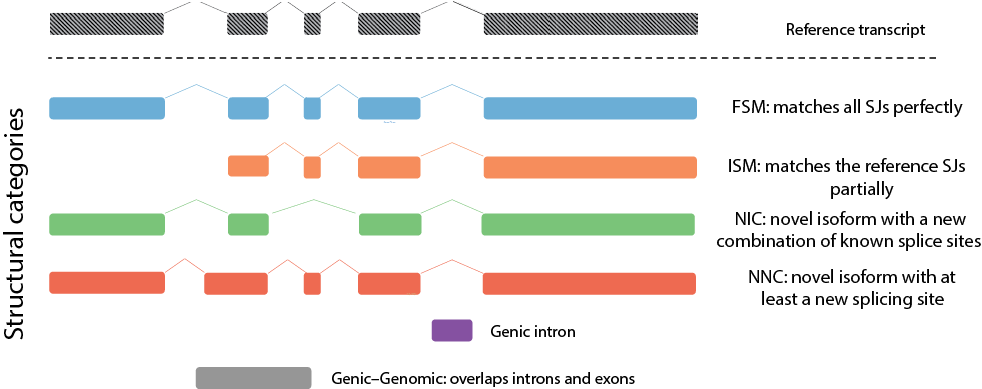
\includegraphics[width=0.9\textwidth]{images/sqanti_structure_category.png}

\end{frame}

\begin{frame}
  \frametitle{Key Features: Unique Junction Chain}
  \centering
  \begin{tikzpicture}[scale=1.15,
      exon/.style={draw, fill=longtrec-blue!50, minimum height=4pt, inner sep=0pt},
      intron/.style={thick, draw=longtrec-blue},
      arrow/.style={-Stealth, thick, color=longtrec-orange},
      every node/.style={font=\scriptsize}]
    
    % Reads with variable TSS/TTS but identical internal junctions
    \def\xA{0}
    \def\xB{1.4}
    \def\xC{2.8}
    \def\xD{4.2}
    
    % Read 1
    \draw[exon] (\xA,0)      rectangle ++(1,0.25);
    \draw[exon] (\xB,0)      rectangle ++(1,0.25);
    \draw[exon] (\xC,0)      rectangle ++(1,0.25);
    \draw[exon] (\xD,0)      rectangle ++(1,0.25);
    \draw[intron] (\xA+1,0.125) .. controls +(0.25,0.4) and +(-0.25,0.4) .. (\xB,0.125);
    \draw[intron] (\xB+1,0.125) .. controls +(0.25,0.4) and +(-0.25,0.4) .. (\xC,0.125);
    \draw[intron] (\xC+1,0.125) .. controls +(0.25,0.4) and +(-0.25,0.4) .. (\xD,0.125);
    \node[anchor=east] at (\xA-0.5,0.125) {Read~1};
    
    % Read 2
    \draw[exon] (\xA-0.3,-0.7) rectangle ++(1.3,0.25);
    \draw[exon] (\xB,-0.7)   rectangle ++(1,0.25);
    \draw[exon] (\xC,-0.7)   rectangle ++(1,0.25);
    \draw[exon] (\xD,-0.7)   rectangle ++(1.3,0.25);
    \draw[intron] (1,-0.575) .. controls +(0.25,0.4) and +(-0.25,0.4) .. (\xB,-0.575);
    \draw[intron] (\xB+1,-0.575) .. controls +(0.25,0.4) and +(-0.25,0.4) .. (\xC,-0.575);
    \draw[intron] (\xC+1,-0.575) .. controls +(0.25,0.4) and +(-0.25,0.4) .. (\xD,-0.575);
    \node[anchor=east] at (\xA-0.5,-0.575) {Read~2};
    
    % Read 3
    \draw[exon] (\xA+0.2,-1.4) rectangle ++(0.8,0.25);
    \draw[exon] (\xB,-1.4)   rectangle ++(1,0.25);
    \draw[exon] (\xC,-1.4)   rectangle ++(1,0.25);
    \draw[exon] (\xD,-1.4)   rectangle ++(0.7,0.25);
    \draw[intron] (1,-1.275) .. controls +(0.25,0.4) and +(-0.25,0.4) .. (\xB,-1.275);
    \draw[intron] (\xB+1,-1.275) .. controls +(0.25,0.4) and +(-0.25,0.4) .. (\xC,-1.275);
    \draw[intron] (\xC+1,-1.275) .. controls +(0.25,0.4) and +(-0.25,0.4) .. (\xD,-1.275);
    \node[anchor=east] at (\xA-0.5,-1.275) {Read~3};

    % Grouping brace
    \draw[decorate,decoration={brace, amplitude=4pt}, thick] (\xD+1.6,0.18) -- (\xD+1.6,-1.42) 
      node[midway,right=4pt,font=\scriptsize] {Same junction chain};

    % Arrow
    \draw[arrow, thick] (\xB+0.5,-1.55) -- (\xB+0.5,-1.9);

    % Collapsed UJC
    \draw[exon, fill=longtrec-orange!50] (\xA,-2.3)   rectangle ++(1,0.25);
    \draw[exon, fill=longtrec-orange!50] (\xB,-2.3)   rectangle ++(1,0.25);
    \draw[exon, fill=longtrec-orange!50] (\xC,-2.3)   rectangle ++(1,0.25);
    \draw[exon, fill=longtrec-orange!50] (\xD,-2.3)   rectangle ++(1,0.25);
    \draw[intron, draw=longtrec-orange!60] (\xA+1,-2.175) .. controls +(0.25,0.35) and +(-0.25,0.35) .. (\xB,-2.175);
    \draw[intron, draw=longtrec-orange!60] (\xB+1,-2.175) .. controls +(0.25,0.35) and +(-0.25,0.35) .. (\xC,-2.175);
    \draw[intron, draw=longtrec-orange!60] (\xC+1,-2.175) .. controls +(0.25,0.35) and +(-0.25,0.35) .. (\xD,-2.175);
    \node[anchor=east] at (\xA-0.5,-2.175) {UJC};
    
    \node[font=\scriptsize, align=center] at (\xB+0.5,-3.1) {
      Reads have variable TSS/TTS but share the same ordered splice junctions.\\
      Such reads collapse into \textbf{one} Unique Junction Chain
    };
  \end{tikzpicture}
\end{frame}

\begin{frame}
  \frametitle{Practical Exercise Overview}
  \begin{columns}[T]
    \begin{column}{0.48\textwidth}
      \textbf{What you'll do:}
      \begin{itemize}
        \item Run alignment workflows with both minimap2 and uLTRA
        \item Compare alignment performance and output quality
        \item Process alignment results through SQANTI-reads
        \item Analyze structural categories and junction patterns
        \item Generate QC reports and visualizations
      \end{itemize}
    \end{column}
    \begin{column}{0.48\textwidth}
      \textbf{Key learning outcomes:}
      \begin{itemize}
        \item Understand trade-offs between different aligners
        \item Grasp the importance of read-level quality control
        \item Learn to interpret SQANTI3 structural categories
        \item Recognize patterns in junction usage across samples
        \item Identify potential technical artifacts in lrRNA-seq data
      \end{itemize}
    \end{column}
  \end{columns}
\end{frame}

%%%%% SECTION: Summary
\section{Summary}

\begin{frame}
  \frametitle{Summary}
  \begin{itemize}
    \item \textbf{Experiment design}: LRGASP Challenge 2 subset focusing on endoderm differentiation markers on chromosome 8
    \item \textbf{Dataset preparation}: Systematic pipeline to extract, process, and validate chromosome 8 reads
    \item \textbf{Alignment comparison}: Hands-on experience with minimap2 (general-purpose) vs uLTRA (RNA-specialized) aligners
    \item \textbf{Quality assessment}: Introduction to SQANTI-reads for comprehensive read-level QC
    \item \textbf{Structural analysis}: Understanding FSM, ISM, NIC, NNC categories and unique junction chains
    \item \textbf{Practical skills}: End-to-end workflow from raw reads to quality-controlled alignments
  \end{itemize}
\end{frame}

% Thank you slide
\thankyouframe{Questions about the practical session?}{https://longtrec.eu}{longtrec@earlham.ac.uk}

\end{document} 